\section{Practical experiment}
In order to validate our system we have developed a practical experiment based on one of the conceptual experiments described in \autoref{chap:sys-arch}.

The base idea of the experiment is to control the speed of the motor using both the local control on the slave device, as shown in \autoref{fig:local-control}, and the remote control concept, as shown in \autoref{fig:remote-control}, where the RTE network is intercalated on the control loop, using a few different configuration values for the network cycle time.

\begin{figure}[htp]
	\centering
	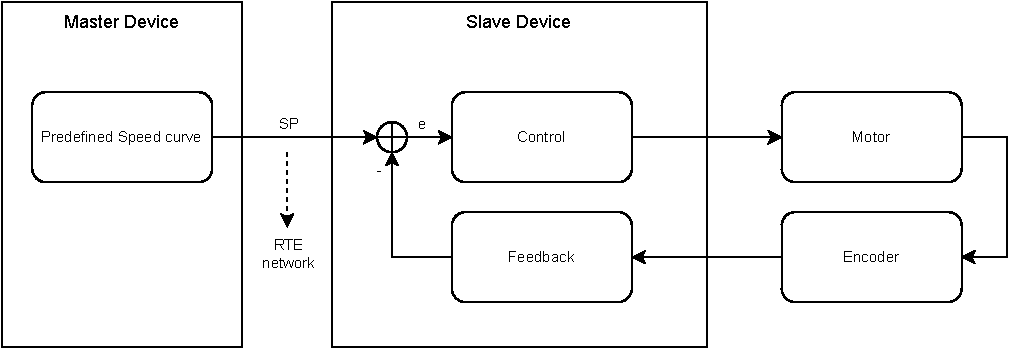
\includegraphics[width=0.8\linewidth]{local-control.pdf}
	\caption{Graph illustrating the local control mode}
	\label{fig:local-control}
\end{figure}

\begin{figure}[htp]
	\centering
	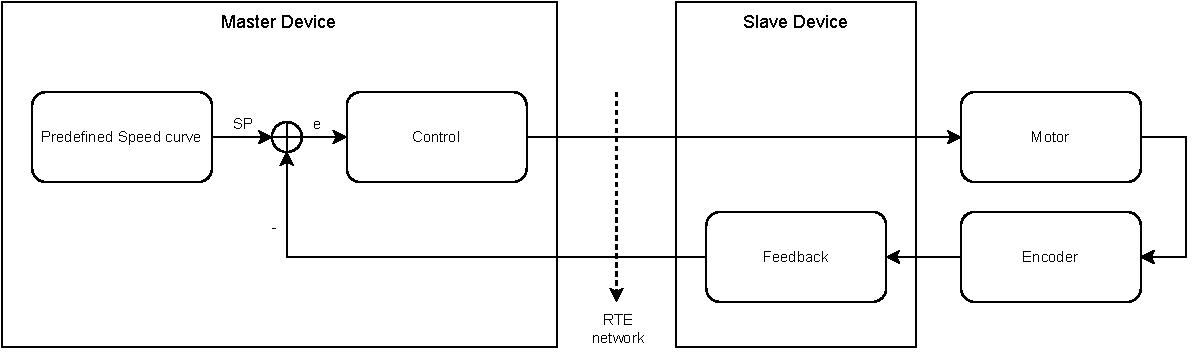
\includegraphics[width=0.8\linewidth]{remote-control.pdf}
	\caption{Graph illustrating the remote control mode}
	\label{fig:remote-control}
\end{figure}

For the local control mode only the set-point values of the speed curve will be transmitted over the RTE network so the expected behaviour is for the network cycle time to barely affect the performance of the speed control loop.
The expected result is for the actual speed of the motor to follow the expected curve with, at most, a small increment to the response time of the process, with the same order of magnitude of the chosen network cycle time.

On the other hand, the remote control mode will have the master node of the RTE network performing the necessary computations and the slave node device will act as a simple networked I/O interface for the system.
This way, the control loop will traverse the slave device and the RTE network before being closed on the master device.
This mode of operation is expected to have a significant impact on the performance of the control loop because the network cycle time will influence the communication delay in both directions.
Not only the plant feedback value will be delayed on its way from the slave device to the master device but also the output value will be delayed on the opposite direction.
This delay is expected to heavily impact the performance of the speed control loop and we expect to obtain either a system with much slower dynamics or, under an extreme condition of network cycle time, a system that might not be controllable.

% speed curve definition
For this experiment we have defined a speed curve comprised of six different stages.
Each stage will set the speed to a single final value, making the set-point preview curve have five step transitions.
The graph shown in \autoref{fig:velocity-curve} has been generated to help visualise the curve.

\begin{figure}[htp]
	\centering
	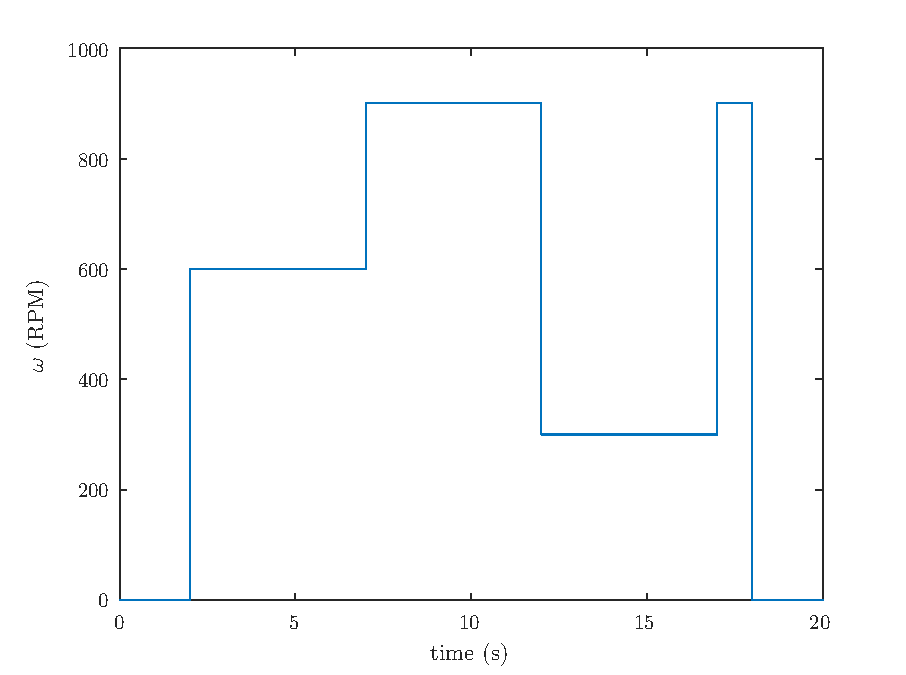
\includegraphics[width=0.8\linewidth]{velocity-curve.pdf}
	\caption{Preview of the defined speed curve}
	\label{fig:velocity-curve}
\end{figure}

This curves evolves as follows:
\begin{enumerate}
	\item two seconds of null speed;
	\item five seconds of 600RPM;
	\item five seconds of 900RPM;
	\item five seconds of 300RPM;
	\item one second of 900RPM;
	\item two seconds of null speed;
\end{enumerate}
We expect this speed curve to provide us with enough variability in both the time and controlled variable domains in order to properly evaluate the system performance in all test cases.

% Network cycle times to use
% `- with a task of 10ms maybe use 5ms, 10ms and 20ms of network cycle time?
Because we intend to implement motion control, we will use a fixed control cycle time of 10ms.
This period will be configured on both the master and slave devices so that value updates occur with the same cadence as the processing.
We will perform three tests with each control mode using three different network cycle periods: 5ms, 10ms and 20ms, which are half, full and double of the control period, respectively.
This effectively means we will present six test cases and compare the performance between local/remote control mode pairs for each network cycle period.

As the system dynamics are expected to change between different test cases, before running each test case the PID controllers will be tuned using the Ziegler-Nichols method \cite{pid:zn-method}.
This defines a procedure to follow in order to determine the controller gains based on the proportional gain that introduces instability ($K_U$) and the frequency/period of oscillation of the system during such instability ($T_U$).
The PID controllers will be tuned with PI configuration, which are the most commonly used for controlling speed.
As such, equations \ref{eq:kp}, \ref{eq:ki} and \ref{eq:kd} show the calculations performed to obtain the tuning values for each test case, presented in \autoref{tab:pid-tunings}.

\begin{equation}
	K_P = 0.45 \cdot K_U
	\label{eq:kp}
\end{equation}

\begin{equation}
	\begin{cases}
		 t_I = \frac{T_U}{1.2} \\
		 K_I = 60 \cdot t_I
	\end{cases}
	\Rightarrow
	K_I = 60 \cdot \frac{T_U}{1.2}
	\label{eq:ki}
\end{equation}

\begin{equation}
	K_D = 0
	\label{eq:kd}
\end{equation}

\begin{table}[htp]
	\centering
	\caption{PID tuning values}
	\label{tab:pid-tunings}
	\begin{tabular}{|c|c|c|c|c|c|c|}
		\hline
		& $K_P$    & $K_I$    & $K_D$    & $K_U$    & $T_U$ (ms)                                  \\
		\hline
		local-5ms   & 0.270    & 1.020    & 0.000    & 0.600    & 20.4                                           \\
		\hline
		remote-5ms  & 0.090    & 0.224    & 0.000    & 0.200    & 50.0                                           \\
		\hline
		local-10ms  & 0.270    & 1.020    & 0.000    & 0.600    & 20.4                                           \\
		\hline
		remote-10ms & 0.081    & 0.238    & 0.000    & 0.180    & 58.8                                           \\
		\hline
		local-20ms  & 0.270    & 1.086    & 0.000    & 0.600    & 21.7                                           \\
		\hline
		remote-20ms & 0.063    & 0.349    & 0.000    & 0.140    & 
		111.0										   \\
		\hline
	\end{tabular}
\end{table}


\subsection{Master node implementation}
In the particular case of this experiment, the master node device is implemented on a generic desktop PC.
It has been programmed using the CODESYS platform and is running on top of Windows 10\texttrademark{}.

The master node device is a home-built desktop computer comprised of an AMD Ryzen\texttrademark{} 5 1600 CPU \cite{hdw:ryzen5-1600}, an MSI X470 Gaming Plus \cite{hdw:msi-x470} motherboard with 2x8 GB dual-channel Kingston HyperX Fury DDR4 RAM (16 GB total) \cite{hdw:hyperx-fury-8gb-ddr4-2400} running at 2400 MHz, a 500 GB Samsung 970 Evo Plus NVMe\textregistered{} M.2 SSD \cite{hdw:970evo-plus-ssd} hard drive, a Gigabyte GeForce\textregistered{} GTX 1650 Super\texttrademark{} OC 4G \cite{hdw:gigabyte-1650-super-oc} graphics card (NVIDIA) and it is powered by an Aerocool KCAS 500W PSU \cite{hdw:kcas-500w}.

The CODESYS platform was used to create a single program on the master node that sends the speed set-points of the predefined speed curve over the RTE network to the slave device, receives the plant feedback values from the RTE network, performs the necessary computations for the control loop and sends the the computed plant output value to the slave node, also through the RTE network.
Because the slave device software ignores the output value arriving on the RTE network interface when it is configured for local control, the same software can be used on the master node for both experiences with local and remote control modes.
Furthermore, this approach makes sure all data to be exported is present on the slave device in both operation modes.

The CODESYS platform includes support to create a Software PLC (SoftPLC) that runs on the desktop PC.
The program is then downloaded to it, as if it was a traditional PLC.
The master device software was implemented in four Program Organisation Unit (POU) implemented in three different IEC 61131-3 programming languages: 
\begin{itemize}
	\item Structured Text (ST) was used in two POUs that perform data type manipulations;
	\item Sequential Function Chart (SFC) was used to program a simple state machine;
	\item Lastly, Function Block Diagram (FBD) was used to map different variables into and out of a PID computation block.
\end{itemize}

The EtherCAT cyclic process data is statically defined as bytes.
As a result, two POUs were programmed in order to convert bytes into \verb|word| (2-byte integer numbers) or \verb|real| (floating point numbers) variables, as necessary.
One such POU will aggregate the input data, arriving from the slave device as bytes, into global variables and the second POU will split the output global variables into bytes.
All relevant variables were created in a Global Variables List (GVL) and the corresponding bytes of the EtherCAT master device are mapped onto these global variables.

The SFC POU implements a simple state machine that controls the time behaviour of the control program and provides a good place where to make the set-point value updates according to the predefined speed curve.
In this case, we followed a minimalist approach to the master device software by hard-coding the timings and set-point values onto the control application.
An overview of the SFC structure can be seen in \autoref{fig:sfc}.

\begin{figure}[htp]
	\centering
	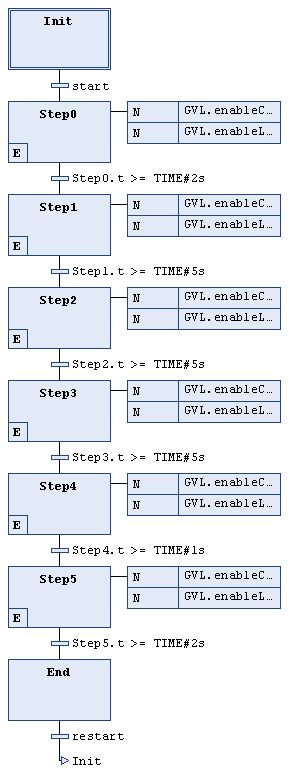
\includegraphics[height=0.6\textheight]{sfc.png}
	\caption{SFC state machine overview}
	\label{fig:sfc}
\end{figure}

At last but not least, the FBD POU maps the required variables onto a PID processing block, to be used during the remote control mode.
The overview of this block can be seen in \autoref{fig:fbd}.

\begin{figure}[htp]
	\centering
	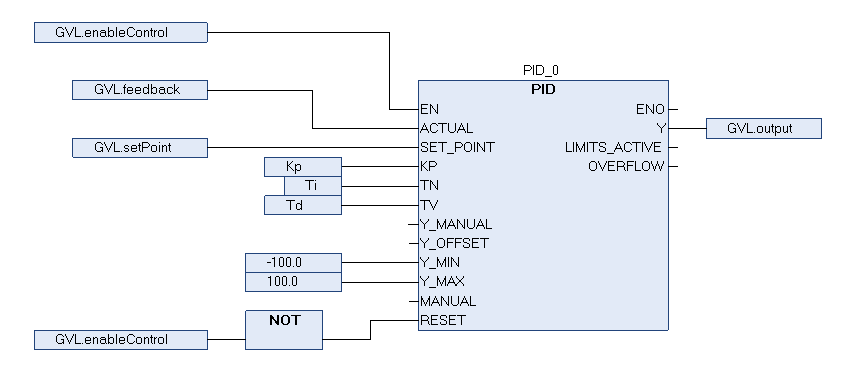
\includegraphics[width=0.8\linewidth]{fbd.png}
	\caption{Overview of the FBD POU}
	\label{fig:fbd}
\end{figure}

\subsection{Slave node configuration}
The slave device requires some configuration parameters to work as expected.
Most importantly, all configurable periods (except for the \verb|enc_period|) will be set to the same value as the control period of the master device, 10ms.
This is to ensure the local and remote control test cases are executed in comparable terms.

The \verb|enc_period| (encoder input polling period) will be left with the default value of 120$\mu$s, to ensure every encoder pulse can be caught even while the motor is running at maximum speed (a motor at 1100RPM with a 360PPR encoder generates one pulse every 151$\mu$s, experimentally we determined a cycle of 120$\mu$s to be able to correctly capture every encoder pulse).

The remaining parameters will be set to: the controlled variable is set to velocity, the PID form is set to position (ignored internally), the PID gains are tuned on each local control test case (when the remote mode is selected these values are ignored) and the remote mode is selected according to each test case.
As a reminder to what was already explained in previous chapters, the slave device parameters are passed to the control application through command-line arguments (refer to \autoref{init-code}).

